\chapter{Data}
In the following chapter, the data used for the validation of the NWCSAF CI product are presented. This includes a description of observations (level 1.5) and products (level 2) from the Meteosat SEVIRI (Spinning Enhanced Visible and Infrared Imager) instrument, as well as the German weather radar composite. Also, an overview of the synoptic conditions is given for the newly considered case days.

\section{Meteosat SEVIRI data}
The Spinning Enhanced Visible and Infrared Imager (SEVIRI) is a passive multispectral imager onboard the geostationary Meteosat Second Generation (MSG) satellites \citep{Schmetz2002}. The SEVIRI instrument has 12 spectral channels covering the visible, near infrared and infrared spectral ranges. The spatial sampling resolution of the channels is \SI{3x3}{\kilo\metre} at nadir, with the exception of the broadband visible HRV channel, which has a nadir spatial resolution of \SI{1x1}{\kilo\metre}. Away from nadir, the spatial resolution decreases due to the increasing viewing zenith angle, reaching about \SI{3x6}{\kilo\metre} and \SI{1x2}{\kilo\metre} for the standard and HRV channels over Europe, respectively. For Europe, SEVIRI data are available in two temporal resolutions. From Meteosat's prime service, a scan of the full earth disk is available every \SI{15}{\minute}, while from the rapid scan service, a scan of the northern-most third of the earth disk is available every \SI{5}{\minute}.

Data from Meteosat's IR~\SI{10.8}{\micro\metre} and HRV channels and from its prime service are used for our evaluation, as the NWC\,SAF CI product calculated based on the prime service was provided for the current study. The use of the rapid scan service for the CI product seems a promising future extension, as it is expected to result in an improved tracking accuracy and thus improved trend calculation.

Additionally, NWC\,SAF cloud property products generated with the v2013 GEO software are utilized for the purposes of parallax correction and the segmentation of cloud fields. Specifically, the NWCSAF  cloud mask (CMa), cloud type (CT), and cloud top temperature and height (CTTH) products are used. In the following, only brief descriptions of these products are given, while more details can be found in \citet{NWCSAFWolken2014}. The choice of v2013 instead of the improved v2016 products was made based on the availability of these products at TROPOS and the short duration of this study. It does however introduce inconsistencies in our study, but its impact is expected to be minor.

The cloud mask (CMa) product is aimed at separating cloud-covered and cloud-free pixels \citep{NWCSAFWolken2014}. The algorithm uses at least four MSG SEVIRI channels together with NWP fields to determine a cloud mask. The algorithm classifies the pixels at the standard SEVIRI spatial resolution into the six classes listed in Tab.~\ref{tab:CMa}.

\begin{table}[htb]
    \centering
    \caption{Class values and corresponding representations of the used NWC\,SAF cloud mask product version}
    \begin{tabular}{rp{0.9\linewidth}}
         \toprule
         class & representation \\
         \midrule
         0 & non processed: no or corrupted data \\
         1 & cloud-free: no contamination by snow or ice and no contamination by clouds \\
         2 & cloud-contaminated: partly cloudy or semitransparent clouds, also dust or volcanic clouds possible \\
         3 & cloud-filled: completely filled by opaque clouds, also thick dust clouds and volcanic plumes included \\
         4 & snow/ice contaminated \\
         5 & undefined: processed but not classified due to known separability problems \\
         \bottomrule
    \end{tabular}
    
    \label{tab:CMa}
\end{table}

Within the scope of this study, only classes 1 and the combination of classes 2 and 3 have been used to separate cloud-free and cloud-containing pixels. 

In addition to the cloud mask, the cloud type (CT) product aims at a detailed analysis of the type of a cloud contained in a pixel \citep{NWCSAFWolken2014}. Using a threshold-based approach considering brightness temperature differences from several SEVIRI IR channels together with the VIS \SI{0.6}{\micro\metre} reflectance, as well as NWP data, clouds are classified into 16 cloud types. For both the v2013 and v2016 versions of the cloud type product, no discrimination of cumuliform and stratiform cloud types is done. The considered cloud types are listed in Tab.~\ref{tab:CT}.

\begin{table}[htp]
    \centering
    \caption{Class values and corresponding representations of the used NWC\,SAF cloud type product version}
    \begin{tabular}{rl}
         \toprule
         class & representation \\
         \midrule
         0 & non-processed: containing no data or corrupted data\\
         1 & cloud-free land \\
         2 & cloud-free sea \\
         3 & land contaminated by snow \\
         4 & sea contaminated by snow/ice \\
         6 & very low clouds \\
         8 & low clouds \\
         10 & medium-level clouds \\
         12 & high opaque clouds \\
         14 & very high opaque clouds \\
         15 & high semitransparent thin clouds \\
         16 & high semitransparent meanly thick clouds \\
         17 & high semitransparent thick clouds clouds \\
         18 & high semitransparent above low or medium clouds \\
         19 & fractional clouds (sub-pixel water clouds) \\
         20 & undefined (undefined by CMa) \\
         \bottomrule
    \end{tabular}
    \label{tab:CT}
\end{table}

It is noteworthy that the CI detection algorithm developed by Mecikalski and co-workers \citep{ MecikalskiBedka2006, MecikalskiBedkaPaechEtAl2008} and adapted to METEOSAT MSG by \citet{MecikalskiMacKenzieKoenigEtAl2010, MecikalskiMacKenzieKoenigEtAl2010a} and \citet{SiewertKoenigMecikalski2010} is known to have problems with cirrus clouds being misclassified as CI and leading to false alarms. Thus all cloudy pixels with a cloud type of semitransparent clouds (cloud type classes 15 to 18) have been excluded from further analyses.

The cloud temperature and height (CTTH) product provides information on the vertical location of a cloud in the atmosphere \citep{NWCSAFWolken2014}. Using at least three MSG SEVIRI channels together with NWP data and the CMa and CT products, the cloud temperature and height are estimated using the RT-TOV radiative transfer model. In the evaluation, the cloud temperature and height product is used for parallax correction of the satellite data for an improved match with weather radar data.

\section{Weather radar data}
\begin{figure}[htbp]
\centering
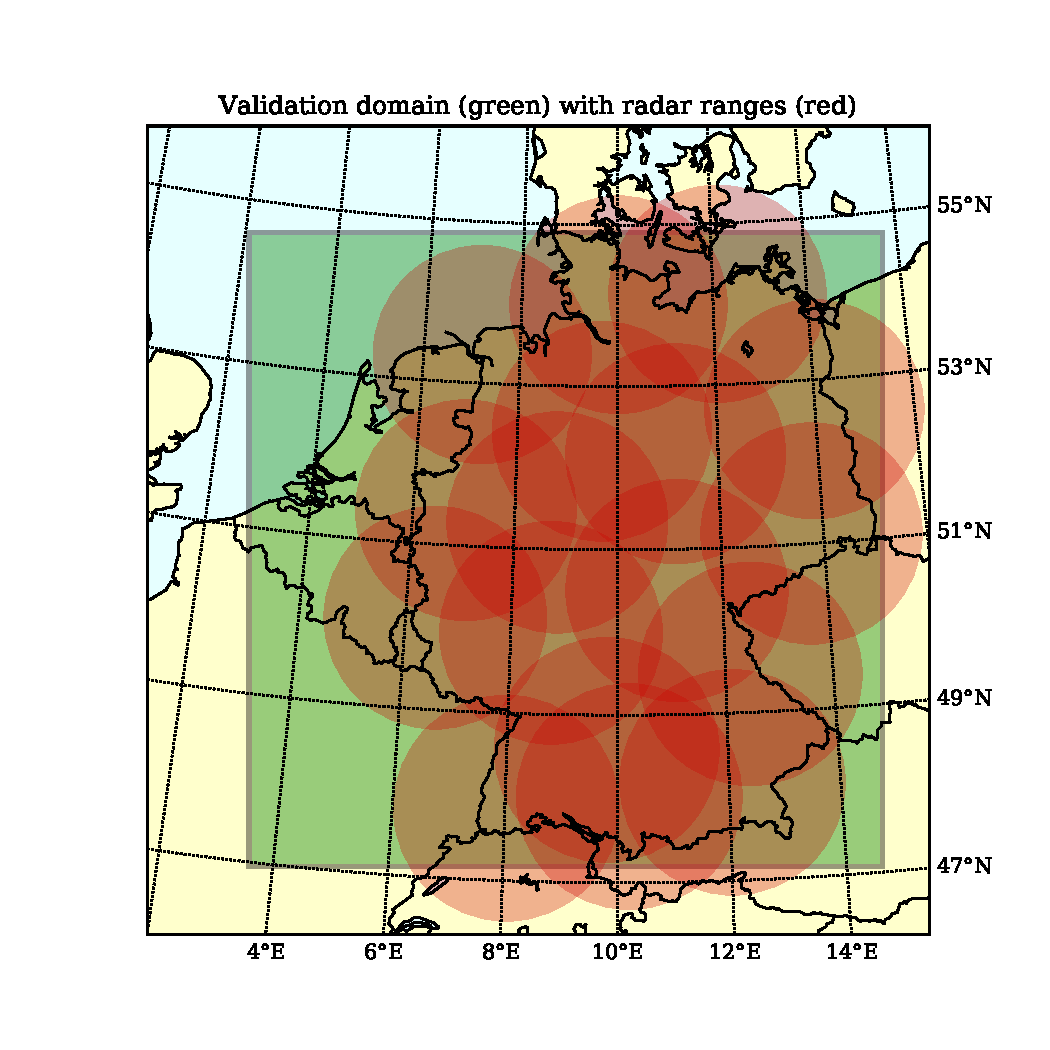
\includegraphics[width=\textwidth]{Grafiken/Abbildungen/radolan_domain.pdf}
\caption{Map of the validation domain (green) with the ranges of the weather radars of the German weather radar network (red). The validation domain is the standard domain of the German weather radar network as defined in \citet{RADOLANkurz2018} and it comprises an area of \SI{900 x 900}{\kilo\metre} covering Germany and parts of its neighbouring countries.}
\label{fig:radolan_domain}
\end{figure}
The validation of the NWC\,SAF CI product is conducted with weather radar data from the RADOLAN RX radar composite, which is used as ground truth for the purposes of our study. The RADOLAN RX radar composite is generated by Deutscher Wetterdienst from observations of the German weather radar network, and is available every five minutes with a spatial resolution of \SI{1 x 1}{\kilo\metre}.  It contains uncorrected radar reflectivity observations and is obtained from 17 C-band radars located throughout Germany with an approximate observing range of \SI{150}{km} each \citep{RADOLANkurz2018}. The domain spans \SI{900 x 900}{\kilo\metre} with a spatial grid resolution of \SI{1 x 1}{\kilo\metre}, and is considered as the validation region for our study. It is shown by the green shaded area in Fig. \ref{fig:radolan_domain}, and comprises Germany, large parts of northeast France, the Netherlands, Luxembourg, large parts of Belgium and smaller parts of Switzerland, Austria, Poland and the Czech Republic. However, the domain is not fully covered by observations, which are shown as red circles in Fig. \ref{fig:radolan_domain}. It also has to be noted that there are relatively frequent outages of individual radars, which affects the quality of the instantaneous products.

\section{Case days}
In the validation study of the NWC\,SAF CI product v2016 by \citet{Karagiannidis2016}, four case days have been considered to validate the product: 25\textsuperscript{th} May 2010, 28\textsuperscript{th} June 2010, 2\textsuperscript{nd} July 2010 and 3\textsuperscript{rd} July 2010. To ensure consistency, three of the four case days are used. As there was no convective development over Germany for 28\textsuperscript{th} June 2010, this day is not considered here. In order to extend the basis for validation, three additional case days were added: 23\textsuperscript{rd} May 2012, 18\textsuperscript{th} June 2013 and 20\textsuperscript{th} June 2013. A synoptic overview of the three additional case days is given below. For a synoptic description of the other three case days, please refer to \citet{Karagiannidis2016}.

\subsection{23\textsuperscript{rd} May 2012}
On 23\textsuperscript{rd} May 2012 large parts of Western and Central Europe are influenced by a pronounced high pressure ridge which extends from the Iberian peninsula until the Baltic Sea (Fig.~\ref{fig:synoptik_20120523}). Corresponding to the high pressure ridge in the middle troposphere a ground high pressure system is located over Scandinavia (Fig.~\ref{fig:synoptik_20120523}a). Over the eastern Atlantic ocean a quite distinct height trough expands from Iceland to the south with several corresponding low pressure systems at the ground. This large scale weather pattern leads to a north eastern flow towards Central Europe. 

Looking at the surface pressure chart (Fig.~\ref{fig:synoptik_20120523}b) it can be seen, that the pressure gradients are relatively low over Western and Central Europe but are stronger along the coasts of the Northern and Baltic Sea along the frontal zone. 

Concerning the GFS reanalysis charts for the KO index / vertical movement (Fig.~\ref{fig:synoptik_20120523}c) and LI/ CAPE (Fig.~\ref{fig:synoptik_20120523}d), it has to be noted that the atmospheric composition is quite unstable which can be seen from the strongly negative values of the KO index. Moreover there are large areas in Central Europe with strong vertical movement induced by the rather high temperatures of the day. Especially over Northern Germany the CAPE is moderately elevated and the LI shows high values, which both indicates a high potential for convective development.

\begin{figure}[htbp]
	\centering
	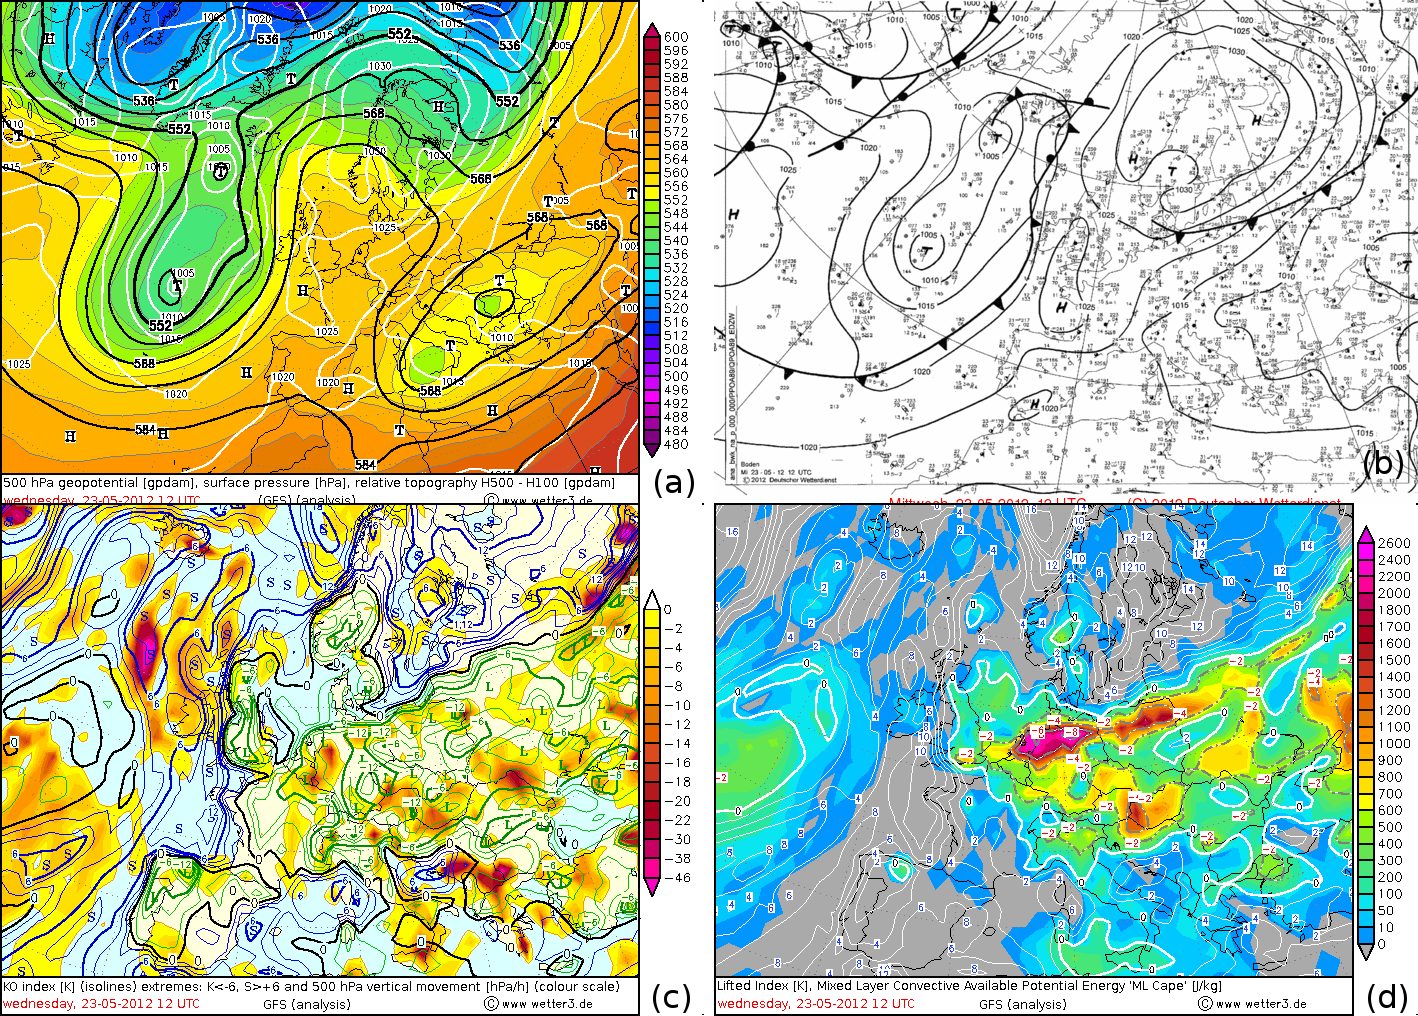
\includegraphics[width=0.8\linewidth]{Grafiken/Abbildungen/synoptik_20120523.png}
	\caption{Synoptic overview for 23\textsuperscript{rd} May 2012, 12:00 UTC, (a) \SI{500}{\hecto\pascal} geopotential, surface pressure and relative topography \SI{500}{\hecto\pascal} - \SI{1000}{\hecto\pascal}, source: www.wetter3.de, (b) Surface pressure analysis, source: Deutscher Wetterdienst, (c) KO index and \SI{500}{\hecto\pascal} vertical movement, source www.wetter3.de, (d) Lifted Index and Mixed Layer Convective Available Potential Energy, source: www.wetter3.de}
    \label{fig:synoptik_20120523}  
\end{figure}

\subsection{18\textsuperscript{th} June 2013}
On 18\textsuperscript{th} June 2013 the weather over Central Europe was dominated by a upper level high pressure ridge which extended from Northern Africa to South West and Central Europe while a upper level trough expanded from Iceland south to the Iberian peninsula where a higher level low pressure core was situated (Fig.~ \ref{fig:synoptik_20130618}a). This large scale weather pattern lead to a southern flow to Central Europe. Along the frontal zone of the upper level low pressure system, hot and unstable air masses where transported northwards leading to an unstable atmospheric composition and a pronounced heat wave over south western Central Europe.

In the ground pressure field several smaller low pressure systems are located below the upper level high pressure ridge, also leading to an unstable atmospheric composition (Fig.~\ref{fig:synoptik_20130618}]b). 

The KO index / vertical movement chart (Fig.~\ref{fig:synoptik_20130618}c) shows strong vertical movements over South West and Central Europe while the KO index is only slightly negative, indicating only a slightly unstable atmosphere. The LI / CAPE chart (Fig.~\ref{fig:synoptik_20130618}d) shows, that strongly elevated CAPE and also strongly negative LI values are present over Central Europe, indicating a strong potential for convective development.

\begin{figure}[htbp]
	\centering
	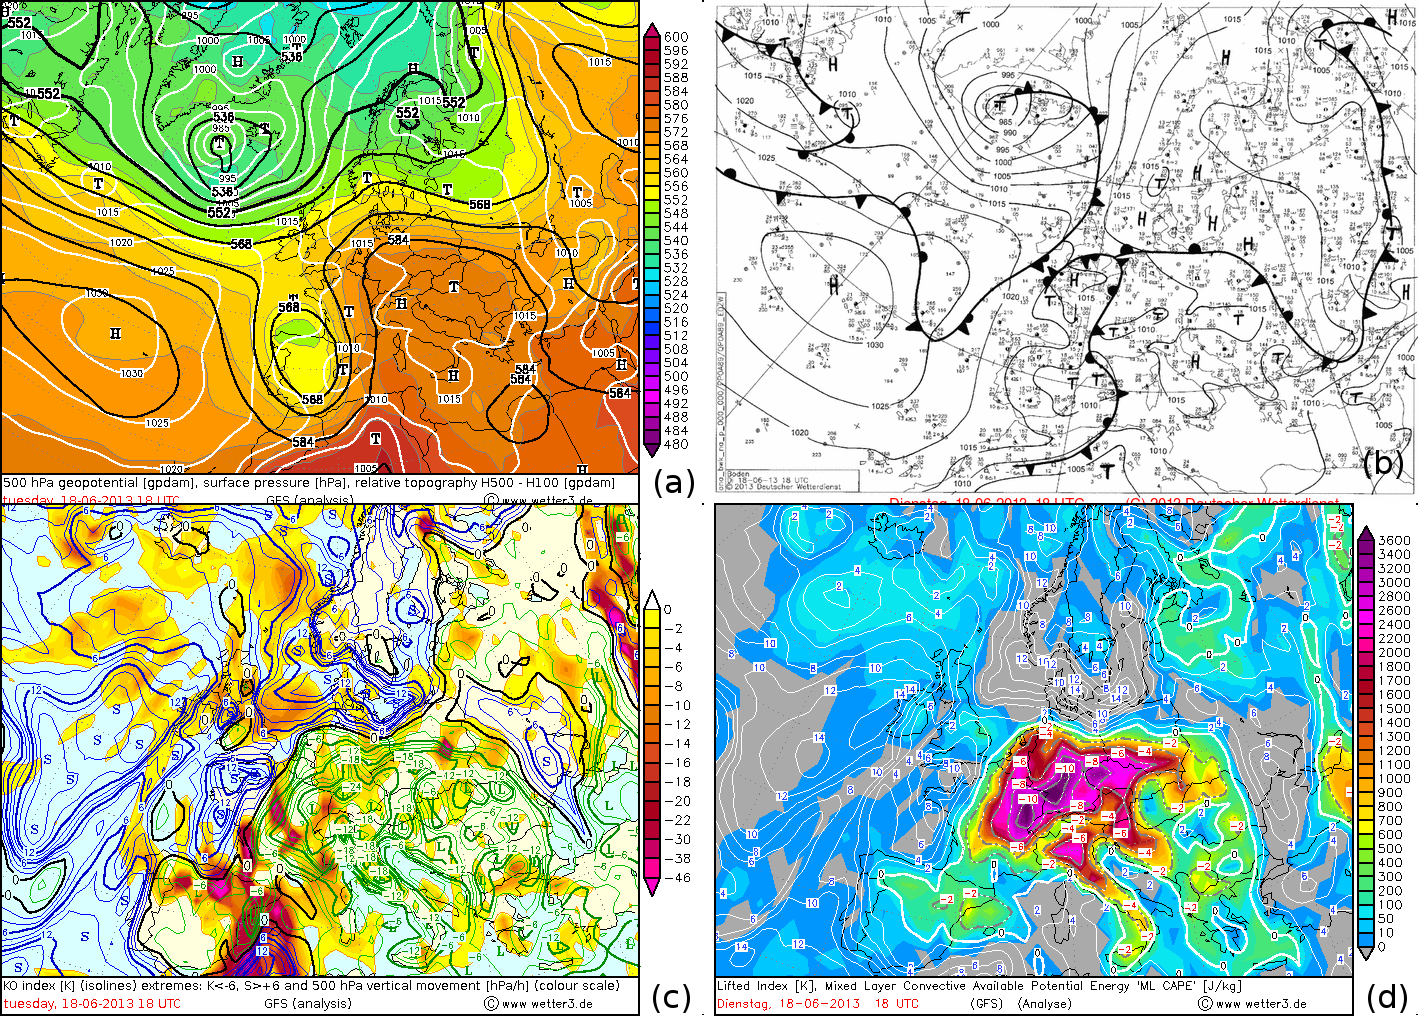
\includegraphics[width=0.8\linewidth]{Grafiken/Abbildungen/synoptik_20130618.png}
	\caption{Same as Fig.~\ref{fig:synoptik_20120523} but for 18\textsuperscript{th} June 2013, 12:00 UTC}
    \label{fig:synoptik_20130618}  
\end{figure}


\subsection{20\textsuperscript{th} June 2013}
The weather situation of the 20\textsuperscript{th} June 2013 was quite similar to the one on 18\textsuperscript{th} June 2013. The large scale weather pattern is similar but the higher level low pressure core situated over Southern France gained more influence on the weather in Central Europe (Fig.~\ref{fig:synoptik_20130620}a). Additionally a heat low pressure system formed in the hot air over North Eastern Germany with a convergence line on its western boundary as can be seen in the ground pressure field (Fig.~\ref{fig:synoptik_20130620}b). Along this convergence line several thunderstorms formed and in the evening the cold front of the low pressure system over Southern France reached Germany leading to the formation an organised thunderstorm line.

The KO index / vertical movement chart (Fig.~\ref{fig:synoptik_20130620}c) shows strong vertical movements over North West Germany and also a strongly negative KO index over this area, indicating a quite unstable atmosphere. The LI / CAPE chart (Fig.~\ref{fig:synoptik_20130620}d) shows, that strongly elevated CAPE and also strongly negative LI values are present over the most parts of Germany, indicating a strong potential for convective development.

\begin{figure}[htbp]
	\centering
	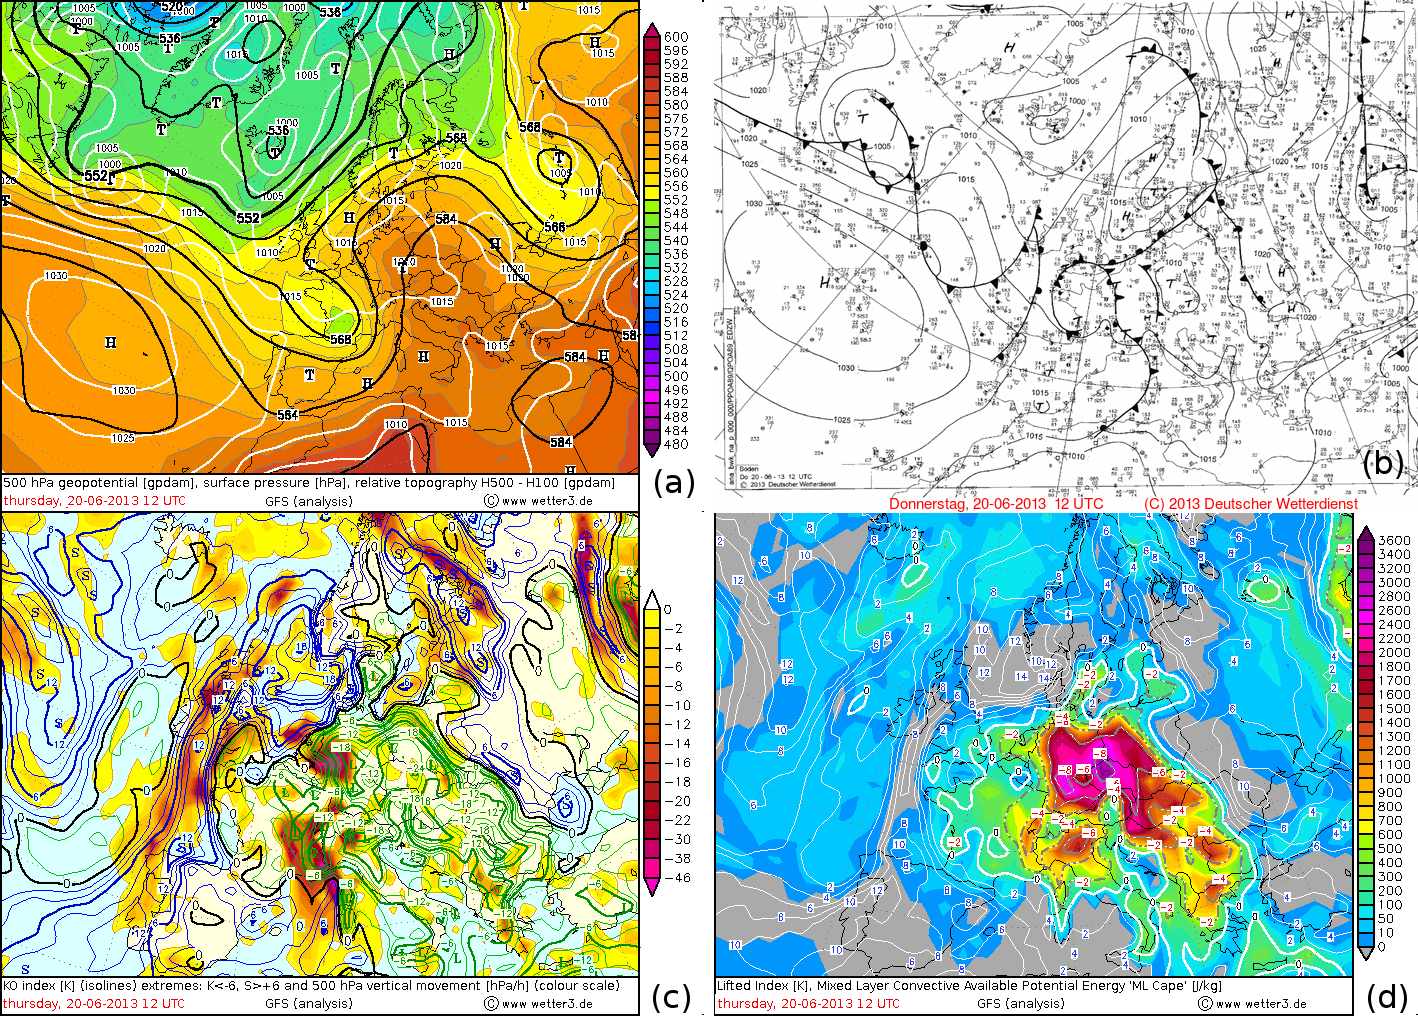
\includegraphics[width=0.8\linewidth]{Grafiken/Abbildungen/synoptik_20130620.png}
	\caption{Same as Fig.~\ref{fig:synoptik_20120523} but for 20\textsuperscript{th} June 2013, 12:00 UTC}
    \label{fig:synoptik_20130620}  
\end{figure}